\section{HadoopDB}
Hadoop  представляет собой платформу для построения приложений, способных обрабатывать огромные объемы данных. 
Система основывается на распределенном подходе к вычислениям и хранению информации, основными ее особенностями являются:
\begin{itemize}
\item \textbf{Масштабируемость:} с помощью Hadoop возможно надежное хранение и обработка огромных объемов данных, 
которые могут измеряться петабайтами;
\item \textbf{Экономичность:} информация и вычисления распределяются по кластеру, построенному на самом 
обыкновенном оборудовании. Такой кластер может состоять из тысяч узлов;
\item \textbf{Эффективность:} распределение данных позволяет выполнять их обработку параллельно на множестве компьютеров, 
что существенно ускоряет этот процесс;
\item \textbf{Надежность:} при хранении данных возможно предоставление избыточности, благодаря хранению нескольких копий. 
Такой подход позволяет гарантировать отсутствие потерь информации в случае сбоев в работе системы;
\item \textbf{Кроссплатформенность:} так как основным языком программирования, используемым в этой системе является Java, 
развернуть ее можно на базе любой операционной системы, имеющей JVM.
\end{itemize}

\textbf{HDFS}

В основе всей системы лежит распределенная файловая система под незамысловатым названием Hadoop 
Distributed File System. Представляет она собой вполне стандартную распределенную файловую систему, но все же 
она обладает рядом особенностей:
\begin{itemize}
\item Устойчивость к сбоям, разработчики рассматривали сбои в оборудовании скорее как норму, чем как исключение;
\item Приспособленность к развертке на самом обыкновенном ненадежном оборудовании;
\item Предоставление высокоскоростного потокового доступа ко всем данным;
\item Настроена для работы с большими файлами и наборами файлов;
\item Простая модель работы с данными: один раз записали~--- много раз прочли;
\item Следование принципу: переместить вычисления проще, чем переместить данные;
\end{itemize}

\textbf{Архитектура HDFS}

\begin{figure}[ht!]
\center{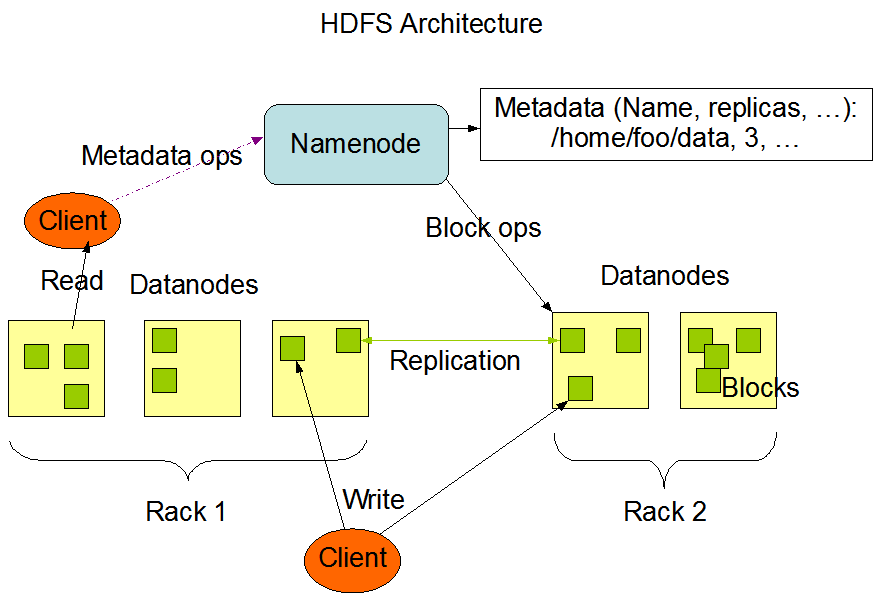
\includegraphics[width=1\textwidth]{hdfsarchitecture}}
\caption{Архитектура HDFS}
\label{fig:hdfsarchitecture}
\end{figure}

\begin{itemize}
\item \textbf{Namenode}

Этот компонент системы осуществляет всю работу с метаданными. Он должен быть запущен только на одном компьютере 
в кластере. Именно он управляет размещением информации и доступом ко всем данным, расположенным на ресурсах кластера. 
Сами данные проходят с остальных машин кластера к клиенту мимо него.

\item \textbf{Datanode}

На всех остальных компьютерах системы работает именно этот компонент. Он располагает сами блоки данных в локальной 
файловой системе для последующей передачи или обработки их по запросу клиента. Группы узлов данных принято называть 
Rack, они используются, например, в схемах репликации данных.

\item \textbf{Клиент}

Просто приложение или пользователь, работающий с файловой системой. В его роли может выступать практически что угодно.
\end{itemize}

Пространство имен HDFS имеет классическую иерархическую структуру: пользователи и приложения имеют возможность 
создавать директории и файлы. Файлы хранятся в виде блоков данных произвольной (но одинаковой, за исключением последнего; 
по-умолчанию 64 mb) длины, размещенных на Datanode'ах. Для обеспечения отказоустойчивости блоки хранятся в нескольких 
экземплярах на разных узлах, имеется возможность настройки количества копий и алгоритма их распределения по системе. 
Удаление файлов происходит не сразу, а через какое-то время после соответствующего запроса, так как после получения 
запроса файл перемещается в директорию /trash и хранится там определенный период времени на случай если пользователь 
или приложение передумают о своем решении. В этом случае информацию можно будет восстановить, в противном случае~--- физически удалить.

Для обнаружения возникновения каких-либо неисправностей, Datanode периодически отправляют Namenode'у сигналы о 
своей работоспособности. При прекращении получения таких сигналов от одного из узлов Namenode помечает его как <<мертвый>>, 
и прекращает какой-либо с ним взаимодействие до возвращения его работоспособности. Данные, хранившиеся на <<умершем>> узле 
реплицируются дополнительный раз из оставшихся <<в живых>> копий и система продолжает свое функционирование как ни в чем не бывало.

Все коммуникации между компонентами файловой системы проходят по специальным протоколам, основывающимся на стандартном TCP/IP. 
Клиенты работают с Namenode с помощью так называемого ClientProtocol, а передача данных происходит по DatanodeProtocol, 
оба они обернуты в Remote Procedure Call (RPC).

Система предоставляет несколько интерфейсов, среди которых командная оболочка DFSShell, набор ПО для администрирования DFSAdmin, 
а также простой, но эффективный веб-интерфейс. Помимо этого существуют несколько API для языков программирования: Java API, 
C pipeline, WebDAV и так далее.

\textbf{MapReduce}

Помимо файловой системы, Hadoop включает в себя framework для проведения масштабных вычислений, обрабатывающих 
огромные объемы данных. Каждое такое вычисление называется Job (задание) и состоит оно, как видно из названия, из двух этапов:

\begin{itemize}
\item \textbf{Map}

Целью этого этапа является представление произвольных данных (на практике чаще всего просто пары ключ-значение) в виде 
промежуточных пар ключ-значение. Результаты сортируются и групируются по ключу и передаются на следующий этап.

\item \textbf{Reduce}

Полученные после map значения используются для финального вычисления требуемых данных. Практические любые данные могут 
быть получены таким образом, все зависит от требований и функционала приложения.
\end{itemize}

Задания выполняются, подобно файловой системе, на всех машинах в кластере (чаще всего одних и тех же). Одна из них выполняет 
роль управления работой остальных — JobTracker, остальные же ее бесприкословно слушаются — TaskTracker. В задачи 
JobTracker'а входит составление расписания выполняемых работ, наблюдение за ходом выполнения, и перераспределение в случае 
возникновения сбоев.

В общем случае каждое приложение, работающее с этим framework'ом, предоставляет методы для осуществления этапов map и reduce, 
а также указывает расположения входных и выходных данных. После получения этих данных JobTracker распределяет задание между 
остальными машинами и предоставляет клиенту полную информацию о ходе работ.

Помимо основных вычислений могут выполняться вспомогательные процессы, такие как составление отчетов о ходе работы, кэширование, 
сортировка и так далее.

\textbf{HBase}

В рамках Hadoop доступна еще и система хранения данных, которую правда сложно назвать СУБД в традиционном смысле этого слова. 
Чаще проводят аналогии с проприетарной системой этого же плана от Google~--- BigTable.

HBase представляет собой распределенную систему хранения больших объемов данных. Подобно реляционным СУБД данные хранятся в 
виде таблиц, состоящих из строк и столбцов. И даже для доступа к ним предоставляется язык запросов HQL (как ни странно~--- 
Hadoop Query Language), отдаленно напоминающий более распространенный SQL. Помимо этого предоставляется итерирующмй интерфейс 
для сканирования наборов строк.

Одной из основных особенностей хранения данных в HBase является возможность наличия нескольких значений, 
соответствующих одной комбинации таблица-строка-столбец, для их различения используется информация о времени добавления записи. 
На концептуальном уровне таблицы обычно представляют как набор строк, но физически же они хранятся по столбцам, достаточно 
важный факт, который стоит учитывать при разработки схемы хранения данных. Пустые ячейки не отображаются каким-либо образом 
физически в хранимых данных, они просто отсутствуют. Существуют конечно и другие нюансы, но я постарался упомянуть лишь основные.

HQL очень прост по своей сути, если Вы уже знаете SQL, то для изучения его Вам понадобится лишь просмотреть по диагонали 
коротенький вывод команды help;, занимающий всего пару экранов в консоли. Все те же SELECT, INSERT, UPDATE, DROP и так далее, 
лишь со слегка измененным синтаксисом.

Помимо обычно командной оболочки HBase Shell, для работы с HBase также предоставлено несколько API для различных языков 
программирования: Java, Jython, REST и Thrift.

\textbf{HadoopDB}

В проекте HadoopDB специалисты из университетов Yale и Brown предпринимают попытку создать гибридную систему управления 
данными, сочетающую преимущества технологий и MapReduce, и параллельных СУБД. В их подходе MapReduce обеспечивает коммуникационную 
инфраструктуру, объединяющую произвольное число узлов, в которых выполняются экземпляры традиционной СУБД. Запросы формулируются 
на языке SQL, транслируются в среду MapReduce, и значительная часть работы передается в экземпляры СУБД. Наличие MapReduce 
обеспечивается масштабируемость и отказоустойчивость, а использование в узлах кластера СУБД позволяет добиться высокой 
производительности. 


\subsection{Установка и настройка}
Вся настройка ведется на Ubuntu Server операционной системе.

\subsubsection{Установка Hadoop}
Перед тем, как приступить собственно говоря к установке Hadoop, необходимо выполнить два элементарных действия, 
необходимых для правильного функционирования системы:
\begin{itemize}
\item открыть доступ одному из пользователей по ssh к этому же компьютеру без пароля, 
можно например создать отдельного пользователя для этого [hadoop]:
\begin{lstlisting}[label=lst:haddop1,caption=Создаем пользователя с правами]
$sudo groupadd hadoop
$sudo useradd -m -g hadoop -d /home/hadoop -s /bin/bash \
-c "Hadoop software owner" hadoop
\end{lstlisting}

Далее действия выполняем от его имени:
\begin{lstlisting}[label=lst:haddop2,caption=Логинимся под пользователем hadoop]
su hadoop
\end{lstlisting}

Генерим RSA-ключ для обеспечения аутентификации в условиях отсутствия возможности использовать пароль:
\begin{lstlisting}[label=lst:haddop3,caption=Генерим RSA-ключ]
hadoop@localhost ~ $ ssh-keygen -t rsa -P ""
Generating public/private rsa key pair.
Enter file in which to save the key (/home/hadoop/.ssh/id_rsa):
Your identification has been saved in /home/hadoop/.ssh/id_rsa.
Your public key has been saved in /home/hadoop/.ssh/id_rsa.pub.
The key fingerprint is:
7b:5c:cf:79:6b:93:d6:d6:8d:41:e3:a6:9d:04:f9:85 hadoop@localhost
\end{lstlisting}

И добавляем его в список авторизованных ключей:
\begin{lstlisting}[label=lst:haddop4,caption=Добавляем его в список авторизованных ключей]
cat $HOME/.ssh/id_rsa.pub >> $HOME/.ssh/authorized_keys
\end{lstlisting}

Этого должно быть более чем достаточно, проверить работоспособность соединения можно просто написав:
\begin{lstlisting}[label=lst:haddop5,caption=Пробуем зайти на ssh без пароля]
ssh localhost
\end{lstlisting}

Не забываем предварительно инициализировать sshd:
\begin{lstlisting}[label=lst:haddop6,caption=Запуск sshd]
/etc/init.d/sshd start
\end{lstlisting}

\item Помимо этого необходимо убедиться в наличии установленной JVM версии 1.5.0 или выше.
\begin{lstlisting}[label=lst:haddop7,caption=Устанавливаем JVM]
sudo aptitude install openjdk-6-jdk
\end{lstlisting}
\end{itemize}

Дальше скачиваем и устанавливаем Hadoop:
\begin{lstlisting}[label=lst:haddop8,caption=Устанавливаем Hadoop]
cd /opt
sudo wget http://www.gtlib.gatech.edu/pub/apache/hadoop
/core/hadoop-0.20.2/hadoop-0.20.2.tar.gz
sudo tar zxvf hadoop-0.20.2.tar.gz
sudo ln -s /opt/hadoop-0.20.2 /opt/hadoop
sudo chown -R hadoop:hadoop /opt/hadoop /opt/hadoop-0.20.2
sudo mkdir -p /opt/hadoop-data/tmp-base
sudo chown -R hadoop:hadoop /opt/hadoop-data/
\end{lstlisting}

Далее переходим в /opt/hadoop/conf/hadoop-env.sh и добавляем вначале:
\begin{lstlisting}[label=lst:haddop9,caption=Указываем переменные окружения]
export JAVA_HOME=/usr/lib/jvm/java-6-openjdk
export HADOOP_HOME=/opt/hadoop
export HADOOP_CONF=$HADOOP_HOME/conf
export HADOOP_PATH=$HADOOP_HOME/bin
export HIVE_HOME=/opt/hive
export HIVE_PATH=$HIVE_HOME/bin

export PATH=$HIVE_PATH:$HADOOP_PATH:$PATH
\end{lstlisting}

Далее добавим в /opt/hadoop/conf/hadoop-site.xml:
\begin{lstlisting}[language=XML,label=lst:haddop10,caption=Настройки hadoop]
<configuration>
<property>
  <name>hadoop.tmp.dir</name>
  <value>/opt/hadoop-data/tmp-base</value>
  <description>A base for other temporary directories</description>
</property>

<property>
  <name>fs.default.name</name>
  <value>localhost:54311</value>
  <description>
    The name of the default file system.
  </description>
</property>

<property>
  <name>hadoopdb.config.file</name>
  <value>HadoopDB.xml</value>
  <description>The name of the HadoopDB 
  cluster configuration file</description>
</property>
</configuration>
\end{lstlisting}

В /opt/hadoop/conf/mapred-site.xml:
\begin{lstlisting}[language=XML,label=lst:haddop11,caption=Настройки mapreduce]
<configuration>
<property>
  <name>mapred.job.tracker</name>
  <value>localhost:54310</value>
  <description>
    The host and port that the 
    MapReduce job tracker runs at.
  </description>
</property>
</configuration>
\end{lstlisting}

В /opt/hadoop/conf/hdfs-site.xml:
\begin{lstlisting}[language=XML,label=lst:haddop12,caption=Настройки hdfs]
<configuration>
<property>
  <name>dfs.replication</name>
  <value>1</value>
  <description>
    Default block replication.
  </description>
</property>
</configuration>
\end{lstlisting}

Теперь необходимо отформатировать Namenode:
\begin{lstlisting}[label=lst:haddop13,caption=Форматирование Namenode]
$ hadoop namenode -format
10/05/07 14:24:12 INFO namenode.NameNode: STARTUP_MSG: 
/************************************************************
STARTUP_MSG: Starting NameNode
STARTUP_MSG:   host = hadoop1/127.0.1.1
STARTUP_MSG:   args = [-format]
STARTUP_MSG:   version = 0.20.2
STARTUP_MSG:   build = https://svn.apache.org/repos
/asf/hadoop/common/branches/branch-0.20 -r
911707; compiled by 'chrisdo' on Fri Feb 19 08:07:34 UTC 2010
************************************************************/
10/05/07 14:24:12 INFO namenode.FSNamesystem: 
fsOwner=hadoop,hadoop
10/05/07 14:24:12 INFO namenode.FSNamesystem: 
supergroup=supergroup
10/05/07 14:24:12 INFO namenode.FSNamesystem: 
isPermissionEnabled=true
10/05/07 14:24:12 INFO common.Storage: 
Image file of size 96 saved in 0 seconds.
10/05/07 14:24:12 INFO common.Storage: 
Storage directory /opt/hadoop-data/tmp-base/dfs/name has been
successfully formatted.
10/05/07 14:24:12 INFO namenode.NameNode: 
SHUTDOWN_MSG: 
/************************************************************
SHUTDOWN_MSG: Shutting down NameNode at hadoop1/127.0.1.1
************************************************************/
\end{lstlisting}

Готово. Теперь мы можем запустить Hadoop:
\begin{lstlisting}[label=lst:haddop14,caption=Запуск Hadoop]
$ start-all.sh
starting namenode, logging to /opt/hadoop/bin/..
/logs/hadoop-hadoop-namenode-hadoop1.out
localhost: starting datanode, logging to 
/opt/hadoop/bin/../logs/hadoop-hadoop-datanode-hadoop1.out
localhost: starting secondarynamenode, logging to
/opt/hadoop/bin/../logs/hadoop-hadoop-secondarynamenode-hadoop1.out
starting jobtracker, logging to 
/opt/hadoop/bin/../logs/hadoop-hadoop-jobtracker-hadoop1.out
localhost: starting tasktracker, logging to
/opt/hadoop/bin/../logs/hadoop-hadoop-tasktracker-hadoop1.out
\end{lstlisting}

Остановка Hadoop производится скриптом stop-all.sh.

\subsubsection{Установка HadoopDB и Hive}
Теперь скачаем HaddopDB\footnote{http://sourceforge.net/projects/hadoopdb/files/} и распакуем hadoopdb.jar в \$HADOOP\_HOME/lib:
\begin{lstlisting}[label=lst:haddop15,caption=Установка HadoopDB]
$cp hadoopdb.jar $HADOOP_HOME/lib
\end{lstlisting}

Также нам потребуется PostgreSQL JDBC библиотека. Скачайте её\footnote{http://jdbc.postgresql.org/download.html} и 
распакуйте в директорию \$HADOOP\_HOME/lib.

Hive используется HadoopDB как SQL интерфейс. Подготовим директорию в HDFS для Hive:
\begin{lstlisting}[label=lst:haddop16,caption=Установка HadoopDB]
hadoop fs -mkdir /tmp
hadoop fs -mkdir /user/hive/warehouse
hadoop fs -chmod g+w /tmp
hadoop fs -chmod g+w /user/hive/warehouse
\end{lstlisting}

В архиве HadoopDB также есть архив SMS\_dist. Распакуем его:
\begin{lstlisting}[label=lst:haddop17,caption=Установка HadoopDB]
tar zxvf SMS_dist.tar.gz
sudo mv dist /opt/hive
sudo chown -R hadoop:hadoop hive
\end{lstlisting}

Поскольку мы успешно запустили Hadoop, то и проблем с запуском Hive не должно быть:
\begin{lstlisting}[label=lst:haddop18,caption=Установка HadoopDB]
$ hive
Hive history file=/tmp/hadoop/
hive_job_log_hadoop_201005081717_1990651345.txt
hive> 

hive> quit;
\end{lstlisting}

\subsubsection{Тестирование}
Теперь проведем тестирование. Для этого скачаем бенчмарк:
\begin{lstlisting}[label=lst:haddop19,caption=Тестирование]
svn co http://graffiti.cs.brown.edu/svn/benchmarks/
cd benchmarks/datagen/teragen
\end{lstlisting}

Изменим скрипт benchmarks/datagen/teragen/teragen.pl к виду:
\begin{lstlisting}[language=Java,label=lst:haddop20,caption=Тестирование]
use strict;
use warnings;

my $CUR_HOSTNAME = `hostname -s`;
chomp($CUR_HOSTNAME);

my $NUM_OF_RECORDS_1TB    = 10000000000;
my $NUM_OF_RECORDS_535MB  = 100;
my $BASE_OUTPUT_DIR   = "/data";
my $PATTERN_STRING    = "XYZ";
my $PATTERN_FREQUENCY = 108299;
my $TERAGEN_JAR       = "teragen.jar";
my $HADOOP_COMMAND    = $ENV{'HADOOP_HOME'}."/bin/hadoop";

my %files = ( "535MB" => 1,
);
system("$HADOOP_COMMAND fs -rmr $BASE_OUTPUT_DIR");
foreach my $target (keys %files) {
my $output_dir = $BASE_OUTPUT_DIR."/SortGrep$target";
my $num_of_maps = $files{$target};
my $num_of_records = ($target eq "535MB" ? 
$NUM_OF_RECORDS_535MB : $NUM_OF_RECORDS_1TB);
print "Generating $num_of_maps files in '$output_dir'\n";

##
## EXEC: hadoop jar teragen.jar 10000000000 
## /data/SortGrep/ XYZ 108299 100
##
my @args = ( $num_of_records,
	    $output_dir,
	    $PATTERN_STRING,
	    $PATTERN_FREQUENCY,
	    $num_of_maps );
my $cmd = "$HADOOP_COMMAND jar $TERAGEN_JAR ".join(" ", @args);
print "$cmd\n";
system($cmd) == 0 || die("ERROR: $!");
} # FOR
exit(0);
\end{lstlisting}

При запуске данного Perl скрипта сгенерится данные, которые будут сохранены на HDFS. 
Поскольку мы настроили систему как единственный кластер, то все данные будут загружены на один HDFS. 
При работе с большим количеством кластеров данные были бы распределены по кластерам.
Создадим базу данных, таблицу и загрузим данные, что мы сохранили на HDFS, в нее:
\begin{lstlisting}[label=lst:haddop21,caption=Тестирование]
$hadoop fs -get /data/SortGrep535MB/part-00000 my_file
$psql
psql> CREATE DATABASE grep0;
psql> USE grep0;
psql> CREATE TABLE grep (
    ->   key1 character varying(255),
    ->   field character varying(255)
    -> );
COPY grep FROM 'my_file' WITH DELIMITER '|';
\end{lstlisting}

Теперь настроим HadoopDB. В архиве HadoopDB можно найти пример файла Catalog.properties. Распакуйт его и настройте:
\begin{lstlisting}[label=lst:haddop22,caption=Тестирование]
#Properties for Catalog Generation
##################################
nodes_file=machines.txt
relations_unchunked=grep, EntireRankings
relations_chunked=Rankings, UserVisits
catalog_file=HadoopDB.xml
##
#DB Connection Parameters
##
port=5432
username=postgres
password=password
driver=com.postgresql.Driver
url_prefix=jdbc\:postgresql\://
##
#Chunking properties
##
chunks_per_node=0
unchunked_db_prefix=grep
chunked_db_prefix=cdb
##
#Replication Properties
##
dump_script_prefix=/root/dump_
replication_script_prefix=/root/load_replica_
dump_file_u_prefix=/mnt/dump_udb
dump_file_c_prefix=/mnt/dump_cdb
##
#Cluster Connection
##
ssh_key=id_rsa
\end{lstlisting}

Создайте файл machines.txt и добавте туда <<localhost>> строчку (без кавычек). Тепер создадим HadoopDB конфиг и скопируем его в HDFS:
\begin{lstlisting}[label=lst:haddop23,caption=Тестирование]
java -cp $HADOOP_HOME/lib/hadoopdb.jar \
> edu.yale.cs.hadoopdb.catalog.SimpleCatalogGenerator \
> Catalog.properties
hadoop dfs -put HadoopDB.xml HadoopDB.xml
\end{lstlisting}

Также возможно создать конфиг для создания репликации командой:
\begin{lstlisting}[label=lst:haddop23:1,caption=Репликация]
java -cp hadoopdb.jar edu.yale.cs.hadoopdb.catalog.SimpleRandomReplicationFactorTwo Catalog.properties
\end{lstlisting}

Инструмент генерирует новый файл HadoopDB.xml, в котором случайные порции данных реплицируются на все узлы.
После этого не забываем обновить конфиг на HDFS:
\begin{lstlisting}[label=lst:haddop23:2,caption=Обновляем конфиг]
hadoop dfs -rmr HadoopDB.xml
hadoop dfs -put HadoopDB.xml HadoopDB.xml
\end{lstlisting}
и поставить <<true>> для <<hadoopdb.config.replication>> в HADOOP\_HOME/conf/hadoop-site.xml.

Теперь мы готовы проверить работы HadoopDB. Теперь можем протестировать поиск по данным, загруженым ранее в БД и HDFS:
\begin{lstlisting}[label=lst:haddop24,caption=Тестирование]
java -cp $CLASSPATH:hadoopdb.jar \
> edu.yale.cs.hadoopdb.benchmark.GrepTaskDB \
> -pattern %wo% -output padraig -hadoop.config.file HadoopDB.xml
\end{lstlisting}

Приблизительный результат:
\begin{lstlisting}[label=lst:haddop25,caption=Тестирование]
$java -cp $CLASSPATH:hadoopdb.jar edu.yale.cs.hadoopdb.benchmark.GrepTaskDB \
> -pattern %wo% -output padraig -hadoop.config.file HadoopDB.xml
14.08.2010 19:08:48 edu.yale.cs.hadoopdb.exec.DBJobBase initConf
INFO: SELECT key1, field FROM grep WHERE field LIKE '%%wo%%';
14.08.2010 19:08:48 org.apache.hadoop.metrics.jvm.JvmMetrics init
INFO: Initializing JVM Metrics with processName=JobTracker, sessionId=
14.08.2010 19:08:48 org.apache.hadoop.mapred.JobClient configureCommandLineOptions
WARNING: Use GenericOptionsParser for parsing the arguments. 
Applications should implement Tool for the same.
14.08.2010 19:08:48 org.apache.hadoop.mapred.JobClient monitorAndPrintJob
INFO: Running job: job_local_0001
14.08.2010 19:08:48 edu.yale.cs.hadoopdb.connector.AbstractDBRecordReader getConnection
INFO: Data locality failed for leo-pgsql
14.08.2010 19:08:48 edu.yale.cs.hadoopdb.connector.AbstractDBRecordReader getConnection
INFO: Task from leo-pgsql is connecting to chunk 0 on host localhost with 
db url jdbc:postgresql://localhost:5434/grep0
14.08.2010 19:08:48 org.apache.hadoop.mapred.MapTask runOldMapper
INFO: numReduceTasks: 0
14.08.2010 19:08:48 edu.yale.cs.hadoopdb.connector.AbstractDBRecordReader close
INFO: DB times (ms): connection = 104, query execution = 20, row retrieval  = 79
14.08.2010 19:08:48 edu.yale.cs.hadoopdb.connector.AbstractDBRecordReader close
INFO: Rows retrieved = 3
14.08.2010 19:08:48 org.apache.hadoop.mapred.Task done
INFO: Task:attempt_local_0001_m_000000_0 is done. And is in the process of commiting
14.08.2010 19:08:48 org.apache.hadoop.mapred.LocalJobRunner$Job statusUpdate
INFO: 
14.08.2010 19:08:48 org.apache.hadoop.mapred.Task commit
INFO: Task attempt_local_0001_m_000000_0 is allowed to commit now
14.08.2010 19:08:48 org.apache.hadoop.mapred.FileOutputCommitter commitTask
INFO: Saved output of task 'attempt_local_0001_m_000000_0' to file:/home/leo/padraig
14.08.2010 19:08:48 org.apache.hadoop.mapred.LocalJobRunner$Job statusUpdate
INFO: 
14.08.2010 19:08:48 org.apache.hadoop.mapred.Task sendDone
INFO: Task 'attempt_local_0001_m_000000_0' done.
14.08.2010 19:08:49 org.apache.hadoop.mapred.JobClient monitorAndPrintJob
INFO:  map 100% reduce 0%
14.08.2010 19:08:49 org.apache.hadoop.mapred.JobClient monitorAndPrintJob
INFO: Job complete: job_local_0001
14.08.2010 19:08:49 org.apache.hadoop.mapred.Counters log
INFO: Counters: 6
14.08.2010 19:08:49 org.apache.hadoop.mapred.Counters log
INFO:   FileSystemCounters
14.08.2010 19:08:49 org.apache.hadoop.mapred.Counters log
INFO:     FILE_BYTES_READ=141370
14.08.2010 19:08:49 org.apache.hadoop.mapred.Counters log
INFO:     FILE_BYTES_WRITTEN=153336
14.08.2010 19:08:49 org.apache.hadoop.mapred.Counters log
INFO:   Map-Reduce Framework
14.08.2010 19:08:49 org.apache.hadoop.mapred.Counters log
INFO:     Map input records=3
14.08.2010 19:08:49 org.apache.hadoop.mapred.Counters log
INFO:     Spilled Records=0
14.08.2010 19:08:49 org.apache.hadoop.mapred.Counters log
INFO:     Map input bytes=3
14.08.2010 19:08:49 org.apache.hadoop.mapred.Counters log
INFO:     Map output records=3
14.08.2010 19:08:49 edu.yale.cs.hadoopdb.exec.DBJobBase run
INFO: 
JOB TIME : 1828 ms.

\end{lstlisting}

Результат сохранен в HDFS, в папке padraig:
\begin{lstlisting}[label=lst:haddop26,caption=Тестирование]
$ cd padraig
$ cat part-00000
some data
\end{lstlisting}

Проверим данные в PostgreSQL:
\begin{lstlisting}[label=lst:haddop27,caption=Тестирование]
psql> select * from grep where field like '%wo%';
+--------------------------------+-------------------+
| key1                           | field
|
+--------------------------------+-------------------+
some data

1 rows in set (0.00 sec)

psql>
\end{lstlisting}

Значения совадают. Все работает как требуется.

Проведем еще один тест. Добавим данные в PostgreSQL:
\begin{lstlisting}[label=lst:haddop27:1,caption=Тестирование]
psql> INSERT into grep(key1, field) VALUES('I am live!', 'Maybe');
psql> INSERT into grep(key1, field) VALUES('I am live!', 'Maybewqe');
psql> INSERT into grep(key1, field) VALUES('I am live!', 'Maybewqesad');
psql> INSERT into grep(key1, field) VALUES(':)', 'May cool string!');
\end{lstlisting}

Теперь проверим через HadoopDB:
\begin{lstlisting}[label=lst:haddop27:2,caption=Тестирование]
$ java -cp $CLASSPATH:hadoopdb.jar edu.yale.cs.hadoopdb.benchmark.GrepTaskDB -pattern %May% -output padraig -hadoopdb.config.file /opt/hadoop/conf/HadoopDB.xml
padraig
01.11.2010 23:14:45 edu.yale.cs.hadoopdb.exec.DBJobBase initConf
INFO: SELECT key1, field FROM grep WHERE field LIKE '%%May%%';
01.11.2010 23:14:46 org.apache.hadoop.metrics.jvm.JvmMetrics init
INFO: Initializing JVM Metrics with processName=JobTracker, sessionId=
01.11.2010 23:14:46 org.apache.hadoop.mapred.JobClient configureCommandLineOptions
WARNING: Use GenericOptionsParser for parsing the arguments. Applications should implement Tool for the same.
01.11.2010 23:14:46 org.apache.hadoop.mapred.JobClient monitorAndPrintJob
INFO: Running job: job_local_0001
01.11.2010 23:14:46 edu.yale.cs.hadoopdb.connector.AbstractDBRecordReader getConnection
INFO: Data locality failed for leo-pgsql
01.11.2010 23:14:46 edu.yale.cs.hadoopdb.connector.AbstractDBRecordReader getConnection
INFO: Task from leo-pgsql is connecting to chunk 0 on host localhost with db url jdbc:postgresql://localhost:5434/grep0
01.11.2010 23:14:47 org.apache.hadoop.mapred.MapTask runOldMapper
INFO: numReduceTasks: 0
01.11.2010 23:14:47 edu.yale.cs.hadoopdb.connector.AbstractDBRecordReader close
INFO: DB times (ms): connection = 181, query execution = 22, row retrieval  = 96
01.11.2010 23:14:47 edu.yale.cs.hadoopdb.connector.AbstractDBRecordReader close
INFO: Rows retrieved = 4
01.11.2010 23:14:47 org.apache.hadoop.mapred.Task done
INFO: Task:attempt_local_0001_m_000000_0 is done. And is in the process of commiting
01.11.2010 23:14:47 org.apache.hadoop.mapred.LocalJobRunner$Job statusUpdate
INFO: 
01.11.2010 23:14:47 org.apache.hadoop.mapred.Task commit
INFO: Task attempt_local_0001_m_000000_0 is allowed to commit now
01.11.2010 23:14:47 org.apache.hadoop.mapred.FileOutputCommitter commitTask
INFO: Saved output of task 'attempt_local_0001_m_000000_0' to file:/home/hadoop/padraig
01.11.2010 23:14:47 org.apache.hadoop.mapred.LocalJobRunner$Job statusUpdate
INFO: 
01.11.2010 23:14:47 org.apache.hadoop.mapred.Task sendDone
INFO: Task 'attempt_local_0001_m_000000_0' done.
01.11.2010 23:14:47 org.apache.hadoop.mapred.JobClient monitorAndPrintJob
INFO:  map 100% reduce 0%
01.11.2010 23:14:47 org.apache.hadoop.mapred.JobClient monitorAndPrintJob
INFO: Job complete: job_local_0001
01.11.2010 23:14:47 org.apache.hadoop.mapred.Counters log
INFO: Counters: 6
01.11.2010 23:14:47 org.apache.hadoop.mapred.Counters log
INFO:   FileSystemCounters
01.11.2010 23:14:47 org.apache.hadoop.mapred.Counters log
INFO:     FILE_BYTES_READ=141345
01.11.2010 23:14:47 org.apache.hadoop.mapred.Counters log
INFO:     FILE_BYTES_WRITTEN=153291
01.11.2010 23:14:47 org.apache.hadoop.mapred.Counters log
INFO:   Map-Reduce Framework
01.11.2010 23:14:47 org.apache.hadoop.mapred.Counters log
INFO:     Map input records=4
01.11.2010 23:14:47 org.apache.hadoop.mapred.Counters log
INFO:     Spilled Records=0
01.11.2010 23:14:47 org.apache.hadoop.mapred.Counters log
INFO:     Map input bytes=4
01.11.2010 23:14:47 org.apache.hadoop.mapred.Counters log
INFO:     Map output records=4
01.11.2010 23:14:47 edu.yale.cs.hadoopdb.exec.DBJobBase run
INFO: 
JOB TIME : 2332 ms.
\end{lstlisting}

Как паттерн поиска я задал <<May>>. В логах можно увидеть как производится поиск. На выходе получаем:
\begin{lstlisting}[label=lst:haddop27:3,caption=Тестирование]
$ cd padraig
$ cat part-00000
I am live!	Maybe
I am live!	Maybewqe
I am live!	Maybewqesad
:)	May cool string!
\end{lstlisting}

В упрощенной системе с одним кластером PostgreSQL не понятно ради чего такие сложности. 
Но если к HadoopDB подключить более одного кластера PostgreSQL, 
то данной методикой возможно работать с данными PostgreSQL, объединенных в shared-nothing кластер.

Более подробно по HadoopDB можно почитать по данной ссылке \\http://hadoopdb.sourceforge.net/guide/quick\_start\_guide.html.


\subsection{Заключение}
В данной статье не показывается, как работать с Hive, как более проще работать с HadoopDB. Эта книга не сможет учесть все, 
что требуется для работы c Hadoop. Назначение этой главы~--- дать основу для работы с Hadoop и HaddopDB.

HadoopDB не заменяет Hadoop. Эти системы сосуществуют, позволяя аналитику выбирать соответствующие средства в зависимости 
от имеющихся данных и задач.

HadoopDB может приблизиться в отношении производительности к параллельным системам 
баз данных, обеспечивая при этом отказоустойчивость и возможность использования в неоднородной среде при тех же правилах 
лицензирования, что и Hadoop. Хотя производительность HadoopDB, вообще говоря, ниже производительности параллельных систем 
баз данных, во многом это объясняется тем, что в PostgreSQL таблицы хранятся не по столбцам, и тем, что в PostgreSQL 
не использовалось сжатие данных. Кроме того, Hadoop и Hive~--- это сравнительно молодые проекты с открытыми кодами. 

В HadoopDB применяется некоторый гибрид подходов параллельных СУБД и Hadoop к анализу данных, позволяющий достичь производительности 
и эффективности параллельных систем баз данных, обеспечивая при этом масштабируемсть, отказоустойчивость и гибкость систем, 
основанных на MapReduce. Способность HadoopDB к прямому включению Hadoop и программного обеспечения СУБД с открытыми исходными 
текстами (без изменения кода) делает HadoopDB особенно пригодной для выполнения крупномасштабного анализа данных в будущих 
рабочих нагрузках.